\hypertarget{stm32f4xx__hal__flash__ramfunc_8c}{}\section{Dokumentacja pliku S\+T\+M/\+W\+D\+S\+\_\+\+Kosc\+\_\+\+Linux/\+Drivers/\+S\+T\+M32\+F4xx\+\_\+\+H\+A\+L\+\_\+\+Driver/\+Src/stm32f4xx\+\_\+hal\+\_\+flash\+\_\+ramfunc.c}
\label{stm32f4xx__hal__flash__ramfunc_8c}\index{S\+T\+M/\+W\+D\+S\+\_\+\+Kosc\+\_\+\+Linux/\+Drivers/\+S\+T\+M32\+F4xx\+\_\+\+H\+A\+L\+\_\+\+Driver/\+Src/stm32f4xx\+\_\+hal\+\_\+flash\+\_\+ramfunc.\+c@{S\+T\+M/\+W\+D\+S\+\_\+\+Kosc\+\_\+\+Linux/\+Drivers/\+S\+T\+M32\+F4xx\+\_\+\+H\+A\+L\+\_\+\+Driver/\+Src/stm32f4xx\+\_\+hal\+\_\+flash\+\_\+ramfunc.\+c}}


F\+L\+A\+SH R\+A\+M\+F\+U\+NC module driver. This file provides a F\+L\+A\+SH firmware functions which should be executed from internal S\+R\+AM.  


{\ttfamily \#include \char`\"{}stm32f4xx\+\_\+hal.\+h\char`\"{}}\newline
Wykres zależności załączania dla stm32f4xx\+\_\+hal\+\_\+flash\+\_\+ramfunc.\+c\+:\nopagebreak
\begin{figure}[H]
\begin{center}
\leavevmode
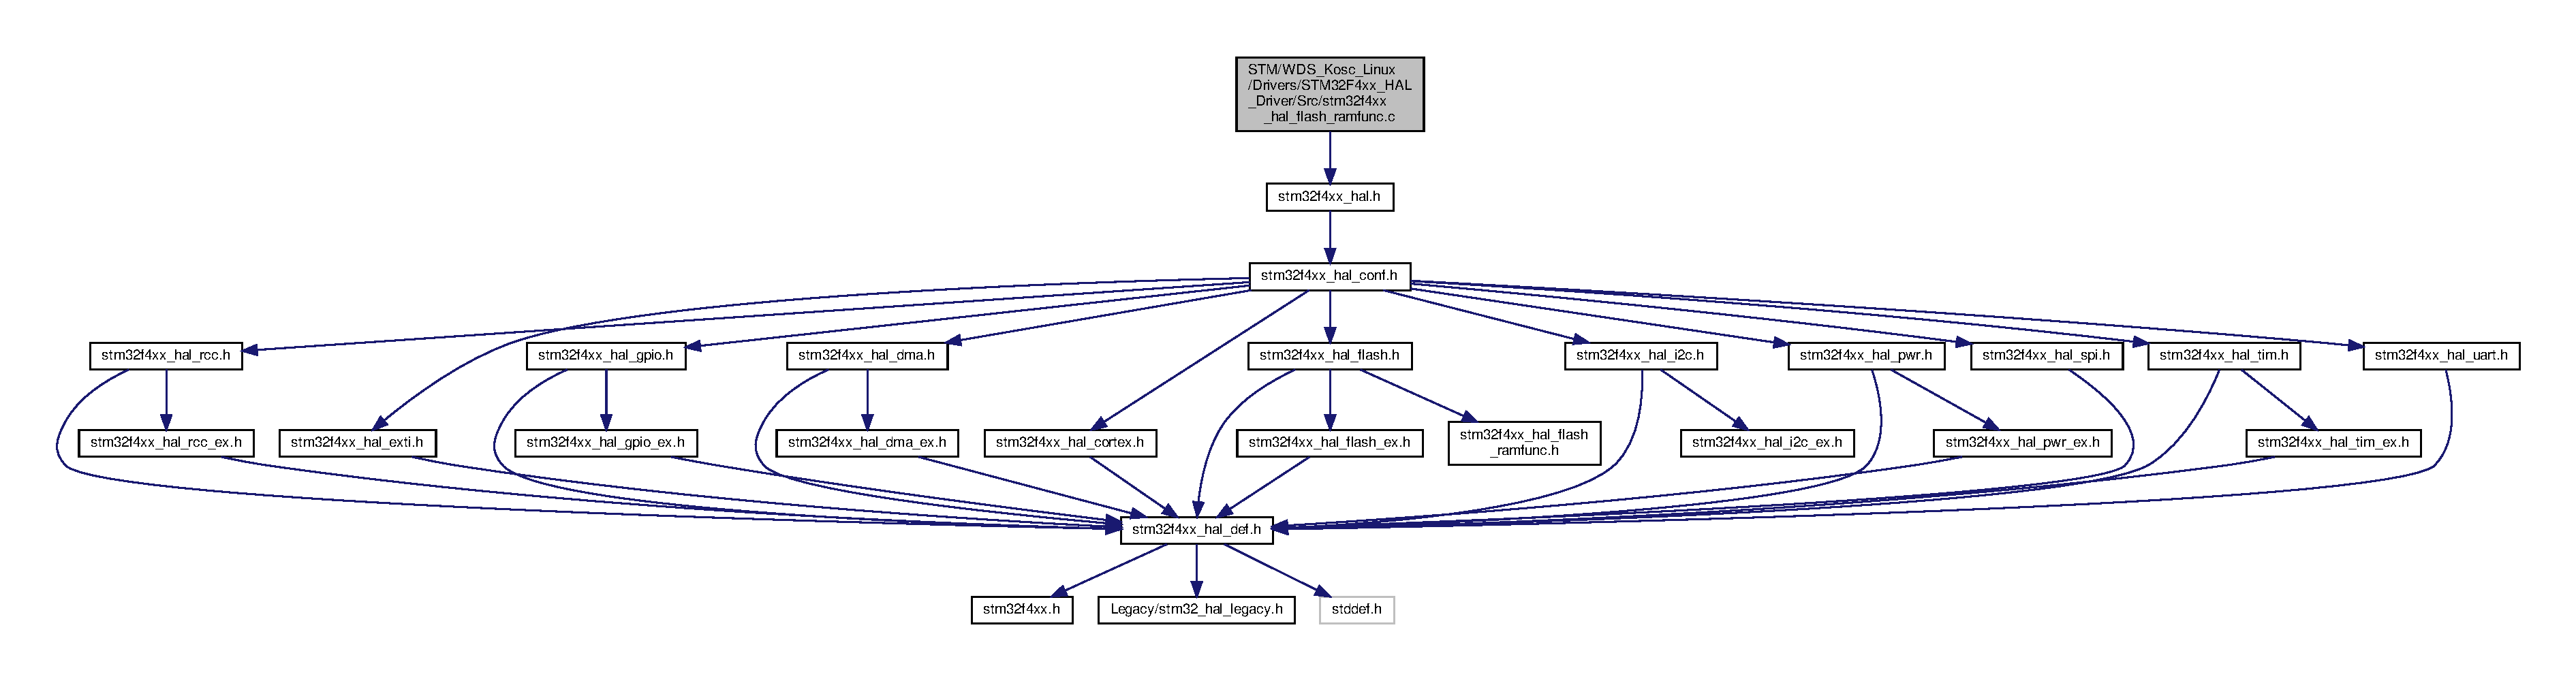
\includegraphics[width=350pt]{stm32f4xx__hal__flash__ramfunc_8c__incl}
\end{center}
\end{figure}


\subsection{Opis szczegółowy}
F\+L\+A\+SH R\+A\+M\+F\+U\+NC module driver. This file provides a F\+L\+A\+SH firmware functions which should be executed from internal S\+R\+AM. 

\begin{DoxyAuthor}{Autor}
M\+CD Application Team
\begin{DoxyItemize}
\item Stop/\+Start the flash interface while System Run
\item Enable/\+Disable the flash sleep while System Run \begin{DoxyVerb}==============================================================================
                  ##### APIs executed from Internal RAM #####
==============================================================================
[..]
  *** ARM Compiler ***
  --------------------
  [..] RAM functions are defined using the toolchain options. 
       Functions that are be executed in RAM should reside in a separate
       source module. Using the 'Options for File' dialog you can simply change
       the 'Code / Const' area of a module to a memory space in physical RAM.
       Available memory areas are declared in the 'Target' tab of the 
       Options for Target' dialog.

  *** ICCARM Compiler ***
  -----------------------
  [..] RAM functions are defined using a specific toolchain keyword "__ramfunc".

  *** GNU Compiler ***
  --------------------
  [..] RAM functions are defined using a specific toolchain attribute
       "__attribute__((section(".RamFunc")))".\end{DoxyVerb}

\end{DoxyItemize}
\end{DoxyAuthor}
\begin{DoxyAttention}{Uwaga}

\end{DoxyAttention}
\subsubsection*{\begin{center}\copyright{} Copyright (c) 2017 S\+T\+Microelectronics. All rights reserved.\end{center} }

This software component is licensed by ST under B\+SD 3-\/\+Clause license, the \char`\"{}\+License\char`\"{}; You may not use this file except in compliance with the License. You may obtain a copy of the License at\+: opensource.\+org/licenses/\+B\+S\+D-\/3-\/\+Clause 